\section{DrawAFriend: The Game}

\begin{figure}
  \centering%
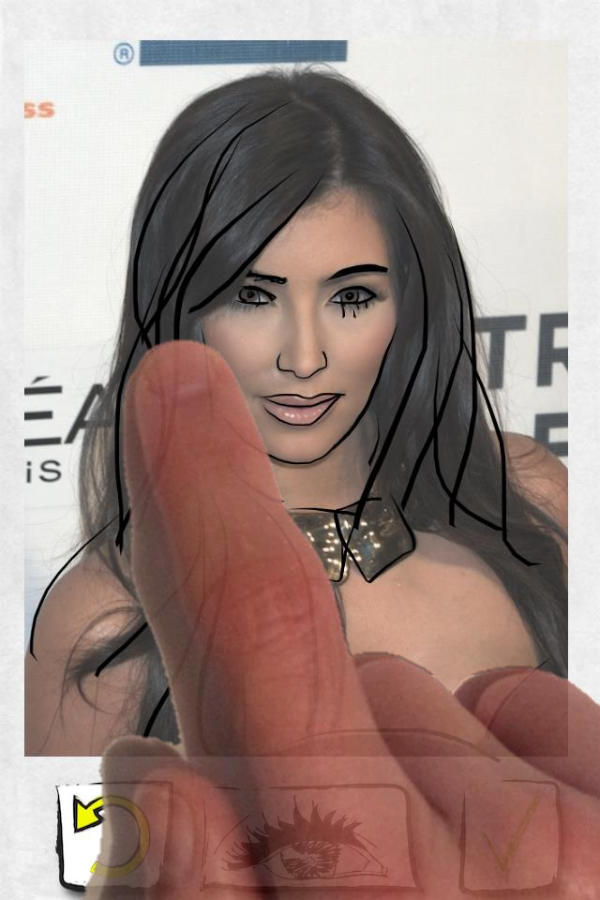
\includegraphics[width=1.5in]{DaF/kim_finger.pdf}
\hspace{0.1in}
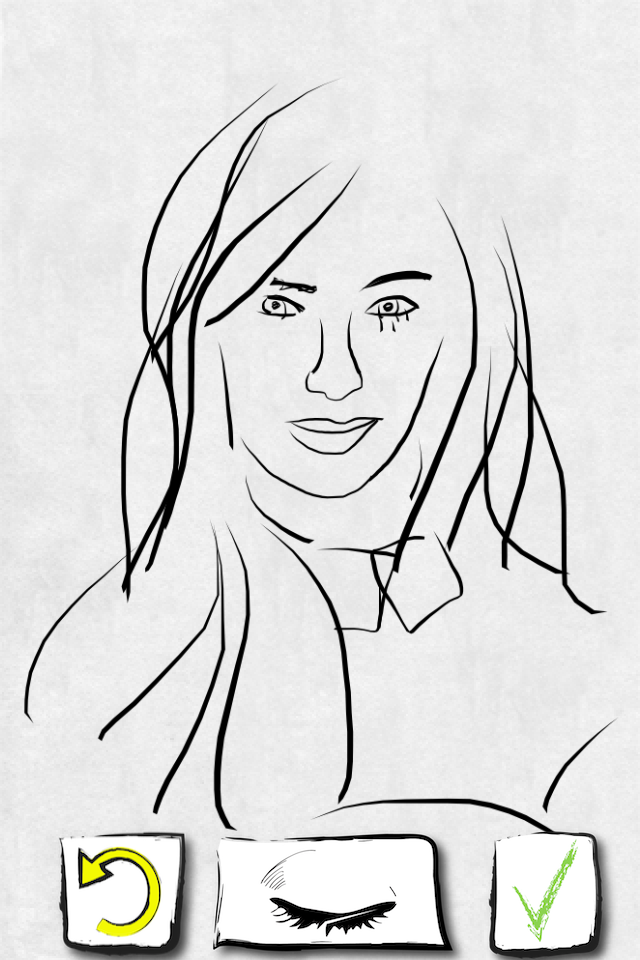
\includegraphics[width=1.5in]{DaF/kim_hidden.png}
  \caption{DrawAFriend: tracing a photo (left), the drawing alone (right).}
  \label{fig:DaF}
\end{figure}

\begin{figure}
  \centering%
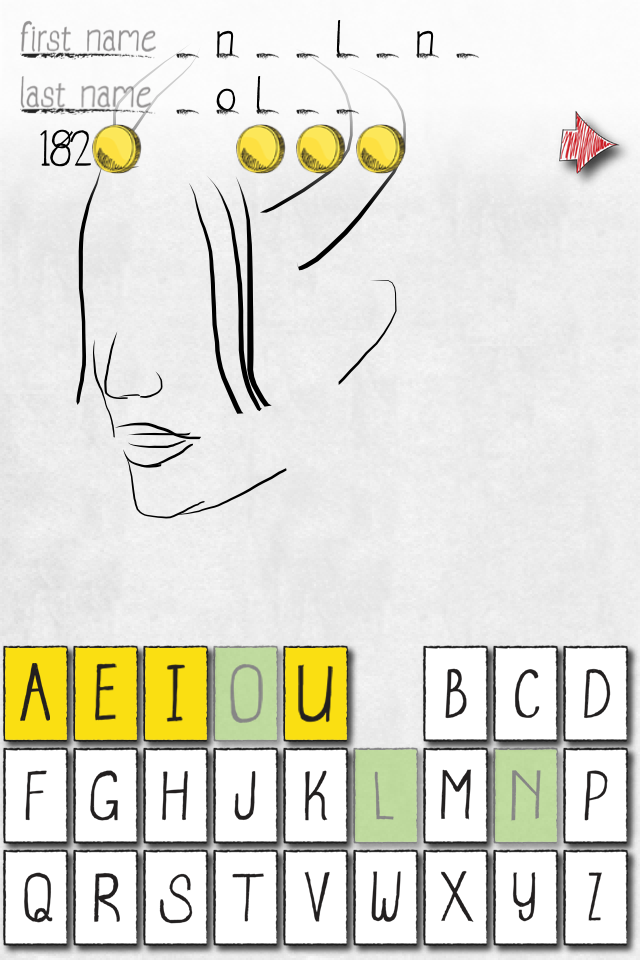
\includegraphics[width=1.5in]{DaF/angelina_guess1.png}
\hspace{0.1in}
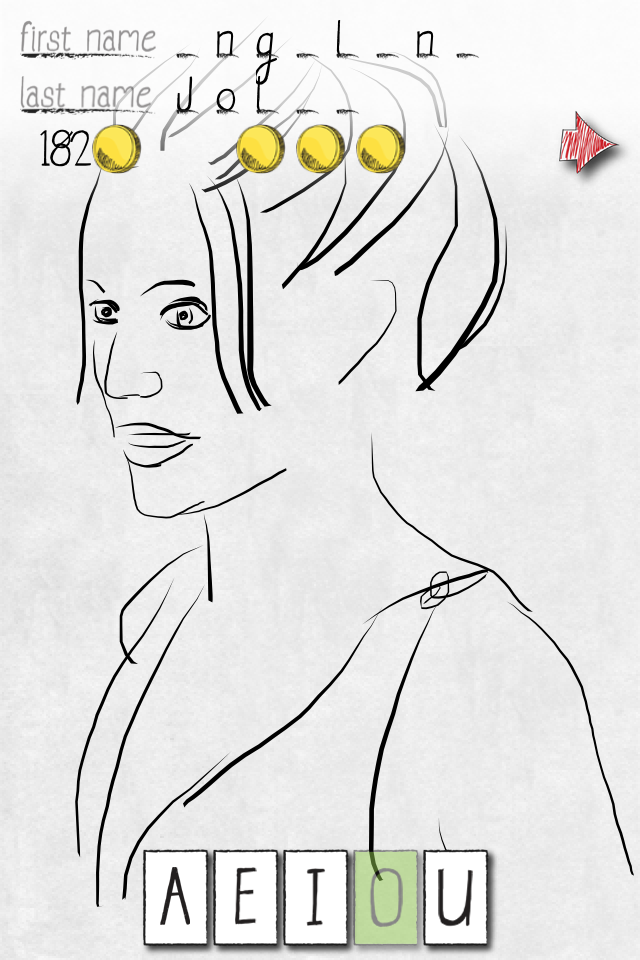
\includegraphics[width=1.5in]{DaF/angelina_guess2.png}
  \caption{DrawAFriend: guessing identity (left). Once a player guesses all consonants in a name, the consonant keys animate away and vowels no longer cost coins. (right).}
  \label{fig:DaF2}
\end{figure}

In order to capture and analyze a large-scale drawing dataset, we have developed \emph{DrawAFriend}, a Facebook-integrated turn-based drawing and guessing game for mobile devices. The game is designed to intrinsically motivate players to contribute drawing through a hangman-like guessing mechanism. This approach enables us to gather a large number of drawings with zero marginal cost per drawing, and to modify and instrument the game to capture specific types of data.

The game works as follows. Players have an option to start a game with either a Facebook friend or an anonymous stranger.  The player is then given four pictures which she can draw. These will either be mutual friends' profile pictures or  celebrity photos. When playing with a stranger, the game offers only celebrity photos.

After choosing a photo to draw, the player is brought to the drawing screen. There she can trace the image (see Figure~\ref{fig:DaF} left). At any point, the user can press the {\em eye} button to hide the photo and see their drawing on its own (Figure~\ref{fig:DaF} right). To overcome the limitations of the phone's size and touch screen inaccuracies, players can pan and zoom using the pinch zoom and two fingered pan gestures.

Once finished, the player sends her drawing to the friend or anonymous player with whom she is playing. The friend receives a notification that they have a drawing to guess. The user is prompted to guess the identity of the other player's drawing (Figure~\ref{fig:DaF2} left). The drawing is replayed stroke by stroke, and similar to {\em Hangman}, the player can guess which letters are in the mutual friend or celebrity's name. Vowels originally cost coins, however once all the consonants are guessed, vowels become free (Figure~\ref{fig:DaF2} right).

The tracing paradigm results in a set of pre-aligned drawings. Whereas other papers begin with rasterized versions of drawings, we collect individual strokes represented as polylines along with timing information.  Furthermore, by observing the guesses we can indirectly evaluate the quality of the drawings. We hypothesize that a good drawing is much more likely to be guessed correctly than a bad drawing. \daf thus leverages a dataset of quality photos (Faceboook profile pictures and celebrity images) and via the efforts of players, results in a large dataset of user created drawings. This dataset includes drawings from artists around the world with different artistic and cultural backgrounds.

For the purposes of tackling the fat finger problem, we focus for the remainder of the paper on the corpus of celebrity drawings. These represent sets of drawings of the same photographs by many different artists.
